\documentclass[a4paper,12pt]{article}
\usepackage{lmodern}
\usepackage{amssymb,amsmath}
\usepackage{ifxetex,ifluatex}
\usepackage{fixltx2e} % provides \textsubscript
\ifnum 0\ifxetex 1\fi\ifluatex 1\fi=0 % if pdftex
  \usepackage[T1]{fontenc}
  \usepackage[utf8]{inputenc}
\else % if luatex or xelatex
  \ifxetex
    \usepackage{mathspec}
  \else
    \usepackage{fontspec}
  \fi
  \defaultfontfeatures{Ligatures=TeX,Scale=MatchLowercase}
\fi
% use upquote if available, for straight quotes in verbatim environments
\IfFileExists{upquote.sty}{\usepackage{upquote}}{}
% use microtype if available
\IfFileExists{microtype.sty}{%
\usepackage{microtype}
\UseMicrotypeSet[protrusion]{basicmath} % disable protrusion for tt fonts
}{}
\usepackage{hyperref}
\hypersetup{unicode=true,
            pdfborder={0 0 0},
            breaklinks=true}
\urlstyle{same}  % don't use monospace font for urls
\usepackage{graphicx,grffile}
\makeatletter
\def\maxwidth{\ifdim\Gin@nat@width>\linewidth\linewidth\else\Gin@nat@width\fi}
\def\maxheight{\ifdim\Gin@nat@height>\textheight\textheight\else\Gin@nat@height\fi}
\makeatother
% Scale images if necessary, so that they will not overflow the page
% margins by default, and it is still possible to overwrite the defaults
% using explicit options in \includegraphics[width, height, ...]{}
\setkeys{Gin}{width=\maxwidth,height=\maxheight,keepaspectratio}
% Make links footnotes instead of hotlinks:
% \renewcommand{\href}[2]{#2\footnote{See \texttt{\url{#1}}}}
\IfFileExists{parskip.sty}{%
\usepackage{parskip}
}{% else
\setlength{\parindent}{0pt}
\setlength{\parskip}{6pt plus 2pt minus 1pt}
}
\setlength{\emergencystretch}{3em}  % prevent overfull lines
\providecommand{\tightlist}{%
  \setlength{\itemsep}{0pt}\setlength{\parskip}{0pt}}
\setcounter{secnumdepth}{5}
% Redefines (sub)paragraphs to behave more like sections
\ifx\paragraph\undefined\else
\let\oldparagraph\paragraph
\renewcommand{\paragraph}[1]{\oldparagraph{#1}\mbox{}}
\fi
\ifx\subparagraph\undefined\else
\let\oldsubparagraph\subparagraph
\renewcommand{\subparagraph}[1]{\oldsubparagraph{#1}\mbox{}}
\fi

\date{}

\usepackage{wrapfig}
\usepackage{enumitem}

%
% Line Spread, Page Markings & Hyperlinked Documents
%
\linespread{1.2}
% Margin:
\usepackage[top=1.5in, bottom=1.5in, right=1in, left=1in]{geometry}

% To silence too small headheight warning
\setlength{\headheight}{15pt}

% Header & Footer:
\usepackage{fancyhdr}
\pagestyle{fancy}
\fancyhf{} % Clear all header and footer fields
\fancyhead[LO,RE]{Helpdesk Ticketing System\\{\vspace{-2pt}\scriptsize Semester 2}}
\fancyhead[LE,RO]{\leftmark\\{\vspace{-4pt}\scriptsize SWE40002 Software Engineering Project}}
\fancyfoot[LE,RO]{\thepage\ifodd\value{page}\else\hfill\fi}
\usepackage{float}

\begin{document}

{
\setcounter{tocdepth}{3}
\tableofcontents
}
\newpage

\begin{minipage}{0.7\textwidth}
\section{Alex Cummaudo}\label{alex-cummaudo}
\begin{itemize}[label={}]
\tightlist
\item
  \textbf{Student Number:} 1744070
\item
  \textbf{Email:}
  \href{mailto:acummaudo@swin.edu.au}{\nolinkurl{acummaudo@swin.edu.au}}
\item
  \textbf{GitHub:} \href{http://www.github.com/alexcu}{alexcu}
\item
  \textbf{Roles:}
  \begin{itemize}
    \item Team Lead
    \item Primary Developer
    \item UX/UI Developer
    \item Documentation
  \end{itemize}
\end{itemize}
\end{minipage}%
\begin{minipage}{0.3\textwidth}
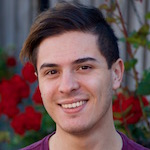
\includegraphics{./imgs/alex.jpeg}
\end{minipage}

\vspace{3em}

\begin{minipage}{0.7\textwidth}
\section{Jake Renzella}\label{jake-renzella}
\begin{itemize}[label={}]
\tightlist
\item
  \textbf{Student Number:} 9993851
\item
  \textbf{Email:}
  \href{mailto:jrenzella@swin.edu.au}{\nolinkurl{jrenzella@swin.edu.au}}
\item
  \textbf{GitHub:}
  \href{http://www.github.com/jakerenzella}{jakerenzella}
\item
  \textbf{Roles:}
  \begin{itemize}
    \item Testing Co-Lead
    \item Project Developer
    \item UX/UI Developer
    \item Documentation
    \item Filming \& Media
  \end{itemize}
\end{itemize}
\end{minipage}%
\begin{minipage}{0.3\textwidth}
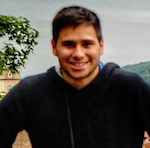
\includegraphics{./imgs/jake.png}
\end{minipage}

\newpage

\begin{minipage}{0.7\textwidth}
\section{Lachlan West}\label{lachlan-west}
\begin{itemize}[label={}]
\tightlist
\item
  \textbf{Student Number:} 2423480
\item
  \textbf{Email:}
  \href{mailto:2423480@student.swin.edu.au}{\nolinkurl{2423480@student.swin.edu.au}}
\item
  \textbf{GitHub:} \href{http://www.github.com/lachlanwest}{lachlanwest}
\item
    \textbf{Roles:}
    \begin{itemize}
      \item Project Developer
      \item Documentation
    \end{itemize}
\end{itemize}
\end{minipage}%
\begin{minipage}{0.3\textwidth}
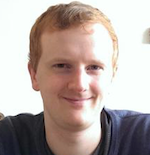
\includegraphics{./imgs/lachy.png}
\end{minipage}

\vspace{3em}

\begin{minipage}{0.7\textwidth}
\section{Reuben Wilson}\label{reuben-wilson}
\begin{itemize}[label={}]
\tightlist
\item
  \textbf{Student Number:} 9988289
\item
  \textbf{Email:}
  \href{mailto:rwilson@swin.edu.au}{\nolinkurl{rwilson@swin.edu.au}}
\item
  \textbf{GitHub:} \href{http://www.github.com/Reubsinit}{Reubsinit}
  \item
    \textbf{Roles:}
    \begin{itemize}
      \item Testing Co-Lead
      \item Project Developer
      \item UX/UI Developer
      \item Documentation
      \item Filming \& Media
    \end{itemize}
\end{itemize}
\end{minipage}%
\begin{minipage}{0.3\textwidth}
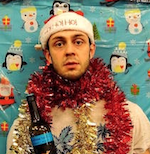
\includegraphics{./imgs/reubs.png}
\end{minipage}

\end{document}
